
%\paragraph*{\color{purple}Context}
Most modern software systems can be customized by means of configuration options to  enable desired functionality or tweak non-functional aspects, such as  performance or energy consumption. The relationship of configuration choices and their influence on performance has been extensively studied in the literature~\cite{dorn2020,siegmundPerformanceinfluenceModelsHighly2015,haDeepPerf2019,perfAL,guoVariabilityawarePerformancePrediction2013,sarkarCostEfficientSamplingPerformance,guo_2018_data,fourier_learning_2015,perLasso,chen_hinnperf_2022}. The backbone of performance estimation are prediction models that map a given configuration to the estimated performance value. Learning performance models relies on a training set of configuration-specific performance measurements. In state-of-the-art approaches, observations usually rely on  only a single workload that aims to represent a typical real-world application scenario.

It is almost folklore that choice of the workload (i.e., the input fed to the software system) influences the performance of software systems in different ways as has been shown for the domains of SAT solving~\cite{falkner_sat_solvers_2015,satzilla_2008}, compilation~\cite{ding_compilation_2015,plotnikov_compilation_2013}, video transcoding~\cite{maxiaguine_workload_2004,alves_sampling_2020}, data compression~\cite{khavari_compression_2019}, and code verification~\cite{koc_satune_2021}. Besides apparent interactions, such as performance scaling with the size of a workload, qualitative aspects can result in intricate and inadvertent performance variations.

{\color{black}
Take as an example two performance throughput distributions across the configuration space of the database \htwo in Figure~\ref{fig:h2_intro}. Here,  the exact same configurations on two different parameterizations of the benchmark \textsf{TPC-C}. have been measured In this scenario, the scale factor controls the modeled number of warehouses. While for most configurations, throughput decreases for a larger benchmark, some configurations achieve even a higher throughput\footnote{A similar example was outlined by~Pereira et al. for the video encoder \xzwo~\cite{alves_sampling_2020}.}. That is, configuration-specific performance can be highly sensitive to workload variation and the behavior under different workloads can change in unforeseeable ways. In turn, this can render performance models based on a single workload useless, unless configuration options’ sensitivity to workloads is accounted for.
}
\begin{figure}
	\centering
	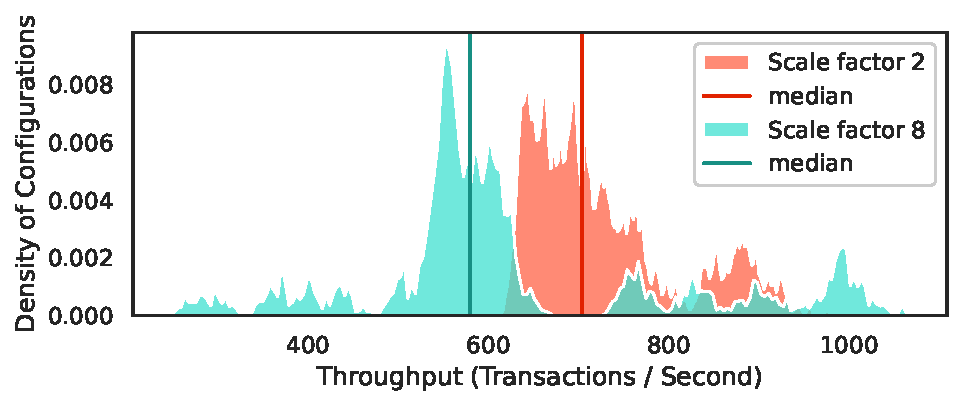
\includegraphics[width=0.99\linewidth]{images/h2_intro.pdf}
	\caption{Throughput distribution of 1\,954 configurations of the database system \htwo run the \textsf{TPC-C} benchmark at different scale factors.}
	\label{fig:h2_intro}
\end{figure}

%\paragraph*{\color{purple}Motivation}
% ~\cite{jamishidi_transfer_2017,jamshidi_learning_2018,jamshidi_transfer_gp_2017}
To address this limitation, two different approaches have been pursued in the literature. 
%First, performance models trained using a specific workload can be adapted to another specific workload. Second,  one can specify workload characteristics as further independent variables when modeling configuration-dependent performance~\cite{koc_satune_2021}.
The first approach relies on transfer learning techniques, where, given an existing performance model, in a separate step only the differences to a new environment are learned. A transfer function encodes which configuration options’ influence on performance is sensitive to workload variation. While transfer learning is an effective strategy that is not limited to varying workloads~\cite{jamshidi_learning_2018,jamishidi_transfer_2017,jamshidi_transfer_gp_2017,martin_transfer_2021,ding_bayesian_2020}, its main limitation is that the transfer function is specific to the differences between two environments.

In contrast to transfer learning, a second and more generalist approach is to consider the input fed to a software system as a further dimension for modeling performance. A workload is characterized by properties that---individually or in conjunction with software configuration options---influence performance. For such a strategy to work, one requires in-depth knowledge of the characteristics of a workload that influence performance. Let alone these characteristics can be mathematically modeled at all. This strategy has been effectively tested for a  variety of application-domains, such as program verification and high-performance computing codes. However, the added complexity comes at significant cost. 
Not only does it require substantially more measurements, we often lack knowledge of which performance-relevant characteristics best describe a workload (e.g., what makes a program hard to verify or optimize).

The existing body of research~\cite{dorn2020,siegmundPerformanceinfluenceModelsHighly2015,haDeepPerf2019,perfAL,guoVariabilityawarePerformancePrediction2013,sarkarCostEfficientSamplingPerformance,guo_2018_data,fourier_learning_2015,perLasso,chen_hinnperf_2022,chen_mmo_2021,nairUsingBadLearners2017,nairFlash18,ohFindingNearoptimalConfigurations2017} confirms the prevalence and importance of the workload influence on software systems. All these works are aware of the workload dimension as a factor of performance variation, yet little is known about the quality and driving factors of the \emph{interplay} between configuration options and workloads. Are workloads and configurations as factors influencing software performance orthogonal and can be treated independently or does their interplay give rise to intricate and inadvertent performance behavior?

We have conducted an empirical study that sheds light on whether and how choices of configuration and workload interact with regard to performance. 
Specifically, we analyzed 25\,258 configurations across nine configurable real-world software systems to obtain a broad picture of the interaction of configuration and workload when learning performance models and estimating a configuration's performance (i.e., response time). Aside from studying the sole effects of workload variation on performance behavior, we explore what is driving the interaction between workload and configuration. To this end, we enrich performance observations with corresponding coverage data to understand workload variation with respect to executed code.

{\color{black}Our findings show that varying the workload can influence con\-fi\-gu\-ra\-tion-de\-pen\-dent software performance in different ways, including non-linear and non-monotonous effects. 
As a \textit{key take-away} of our study, we found empirical evidence that single-workload approaches do not generalize across workload variations and that even existing transfer learning techniques are too limited to address non-monotonous performance variations induced by qualitative workload changes. 
}

To summarize, we make the following contributions: 
\begin{compactitem}
	\item An empirical study of 25\,258 configurations across nine configurable software systems on whether and how interactions of workload and configuration affect software  performance;
	
	\item {\color{red}A detailed analysis that illustrates that variation in code coverage due to varying workloads can affect the influence of individual configuration options on software performance; }
	
	\item A companion Web site\footnote{\color{red}TODO: move supplementary web site to gitlab} with supplementary material including performance and coverage measurements, experiment workloads and configurations, and an interactive dashboard\footnote{\url{https://workload-performance.herokuapp.com}} for data exploration to \textit{reproduce} all analyses and additional visualizations left out due to space limitations.
	
\end{compactitem}


